\documentclass{article}\usepackage[]{graphicx}\usepackage[]{color}
% maxwidth is the original width if it is less than linewidth
% otherwise use linewidth (to make sure the graphics do not exceed the margin)
\makeatletter
\def\maxwidth{ %
  \ifdim\Gin@nat@width>\linewidth
    \linewidth
  \else
    \Gin@nat@width
  \fi
}
\makeatother

\definecolor{fgcolor}{rgb}{0.345, 0.345, 0.345}
\newcommand{\hlnum}[1]{\textcolor[rgb]{0.686,0.059,0.569}{#1}}%
\newcommand{\hlstr}[1]{\textcolor[rgb]{0.192,0.494,0.8}{#1}}%
\newcommand{\hlcom}[1]{\textcolor[rgb]{0.678,0.584,0.686}{\textit{#1}}}%
\newcommand{\hlopt}[1]{\textcolor[rgb]{0,0,0}{#1}}%
\newcommand{\hlstd}[1]{\textcolor[rgb]{0.345,0.345,0.345}{#1}}%
\newcommand{\hlkwa}[1]{\textcolor[rgb]{0.161,0.373,0.58}{\textbf{#1}}}%
\newcommand{\hlkwb}[1]{\textcolor[rgb]{0.69,0.353,0.396}{#1}}%
\newcommand{\hlkwc}[1]{\textcolor[rgb]{0.333,0.667,0.333}{#1}}%
\newcommand{\hlkwd}[1]{\textcolor[rgb]{0.737,0.353,0.396}{\textbf{#1}}}%
\let\hlipl\hlkwb

\usepackage{framed}
\makeatletter
\newenvironment{kframe}{%
 \def\at@end@of@kframe{}%
 \ifinner\ifhmode%
  \def\at@end@of@kframe{\end{minipage}}%
  \begin{minipage}{\columnwidth}%
 \fi\fi%
 \def\FrameCommand##1{\hskip\@totalleftmargin \hskip-\fboxsep
 \colorbox{shadecolor}{##1}\hskip-\fboxsep
     % There is no \\@totalrightmargin, so:
     \hskip-\linewidth \hskip-\@totalleftmargin \hskip\columnwidth}%
 \MakeFramed {\advance\hsize-\width
   \@totalleftmargin\z@ \linewidth\hsize
   \@setminipage}}%
 {\par\unskip\endMakeFramed%
 \at@end@of@kframe}
\makeatother

\definecolor{shadecolor}{rgb}{.97, .97, .97}
\definecolor{messagecolor}{rgb}{0, 0, 0}
\definecolor{warningcolor}{rgb}{1, 0, 1}
\definecolor{errorcolor}{rgb}{1, 0, 0}
\newenvironment{knitrout}{}{} % an empty environment to be redefined in TeX

\usepackage{alltt}

\usepackage[dvipsnames]{xcolor}
\usepackage[margin=1.0in]{geometry}
\usepackage[pdftex]{lscape}

\usepackage{amssymb}
\usepackage{array}
\usepackage{fancyhdr}
\usepackage{float}
\usepackage{graphicx}
\usepackage{listings}
\usepackage{longtable}
\usepackage{moreverb}
\usepackage{multirow}
\usepackage{setspace}
\usepackage{tabularx}
\usepackage{threeparttable}
\usepackage{verbatim}

\usepackage[backend=biber, natbib, style=authoryear-icomp,doi=false,isbn=false,url=false]{biblatex}
\addbibresource{$BIB}

\definecolor{codegreen}{rgb}{0,0.6,0}
\definecolor{codegray}{rgb}{0.5,0.5,0.5}
\definecolor{codepurple}{rgb}{0.58,0,0.82}
\definecolor{backcolour}{rgb}{0.95,0.95,0.92}

\lstdefinestyle{mystyle}{
    backgroundcolor=\color{backcolour},
    commentstyle=\color{codegreen},
    keywordstyle=\color{magenta},
    numberstyle=\scriptsize\color{codegray},
    stringstyle=\color{codepurple},
    basicstyle=\ttfamily\scriptsize,
    breakatwhitespace=false,
    breaklines=true,
    captionpos=b,
    keepspaces=true,
    numbers=left,
    numbersep=5pt,
    showspaces=false,
    showstringspaces=false,
    showtabs=false,
    tabsize=2
}

\lstset{style=mystyle}
\newenvironment{centerfig}
{\begin{figure}[H]\centering}
{\end{figure}}

\renewcommand\maketitle{}
\title{POLS0012 Final}
\author{}
\IfFileExists{upquote.sty}{\usepackage{upquote}}{}
\begin{document}
\maketitle



\section{Part A: Quantatative Questions}
\subsection{Question 1}


\subsubsection{Part 1}


The mean difference in enforcement of detainer requests is -1.7\%.
Compared to republican sheriffs, democratic sheriffs comply with detainer requests 1.7 percentage points less of the time.

This 1.7\% estimate cannot be interpreted as a causal effect as the two groups we are comparing are systematically different from each other and cannot be thought of as plausible counterfactuals of one another.

As an illustration of the problem, rural counties generally have more republican voters \parencite[][]{Gimpel_2020}.
If rural counties are also more likely to respond to detainer requests for any reason, then the difference in group means could be a reflection of this causal relationship rather than a link between the election of a republican and a change in the proportion of detainer requests processed.

\subsubsection{Part 2}
A regression discontinuity design (RDD) allows us to estimate the causal effect of electing a democratic sheriff by focusing on a group of counties that are comparable: the most marginal elections where the election was decided by a slim margin.
We assume that these elections were decided in an ``as good as random" manner. If this is the case, then the units that fall just on one side and just on the other side of a cutoff are plausible counterfactuals of one another \parencite[][]{McCrary_2008}, and can be directly compared to find the causal effect.

\subsubsection{Part 3}
I create the running variable and add it to the data used with the regression.
The code used can be seen below:

\begin{knitrout}
\definecolor{shadecolor}{rgb}{0.969, 0.969, 0.969}\color{fgcolor}\begin{kframe}
\begin{alltt}
\hlcom{#Question 1 Part 3}
\hlstd{sheriff_data} \hlkwb{<-} \hlstd{sheriff_data} \hlopt \hlkwd{mutate}\hlstd{(}\hlstr{"running_var"} \hlstd{= dem_vote_share} \hlopt{-} \hlnum{50.0}\hlstd{)}
\end{alltt}
\end{kframe}
\end{knitrout}

\subsubsection{Part 4}
The key assumption of an RDD design is that the treatment assignment is as-good-as-random at the cutoff.
If units are allowed to sort into the treatment or control groups this means that the randomization has failed.
A selection bias is introduced, and the treated and untreated groups are no longer directly comparable.

As \citet{Caughey_2011} have shown with respect to U.S. House elections, close elections do not always guarantee randomization.
I test whether barely elected sheriffs are more likely to be incumbents using another RDD and find no significant effect. This gives no evidence to suggest sorting.

The McCrary test \parencite[][]{McCrary_2008} can also effectively test for sorting by looking for discontinuity in the distribution of the running variable.
A p-value of .454 from this test means that we do not have significant evidence to reject the null hypothesis of continuity at the cutoff.
In other words, we do not have evidence to suggest that there is any discontinuity or sorting at the cutoff value.
This can also be seen in the plot of the density estimate of the running variable, which is continuous at the cutoff.

\begin{centerfig}
\caption{Density estimate of the running variable}
\begin{knitrout}
\definecolor{shadecolor}{rgb}{0.969, 0.969, 0.969}\color{fgcolor}
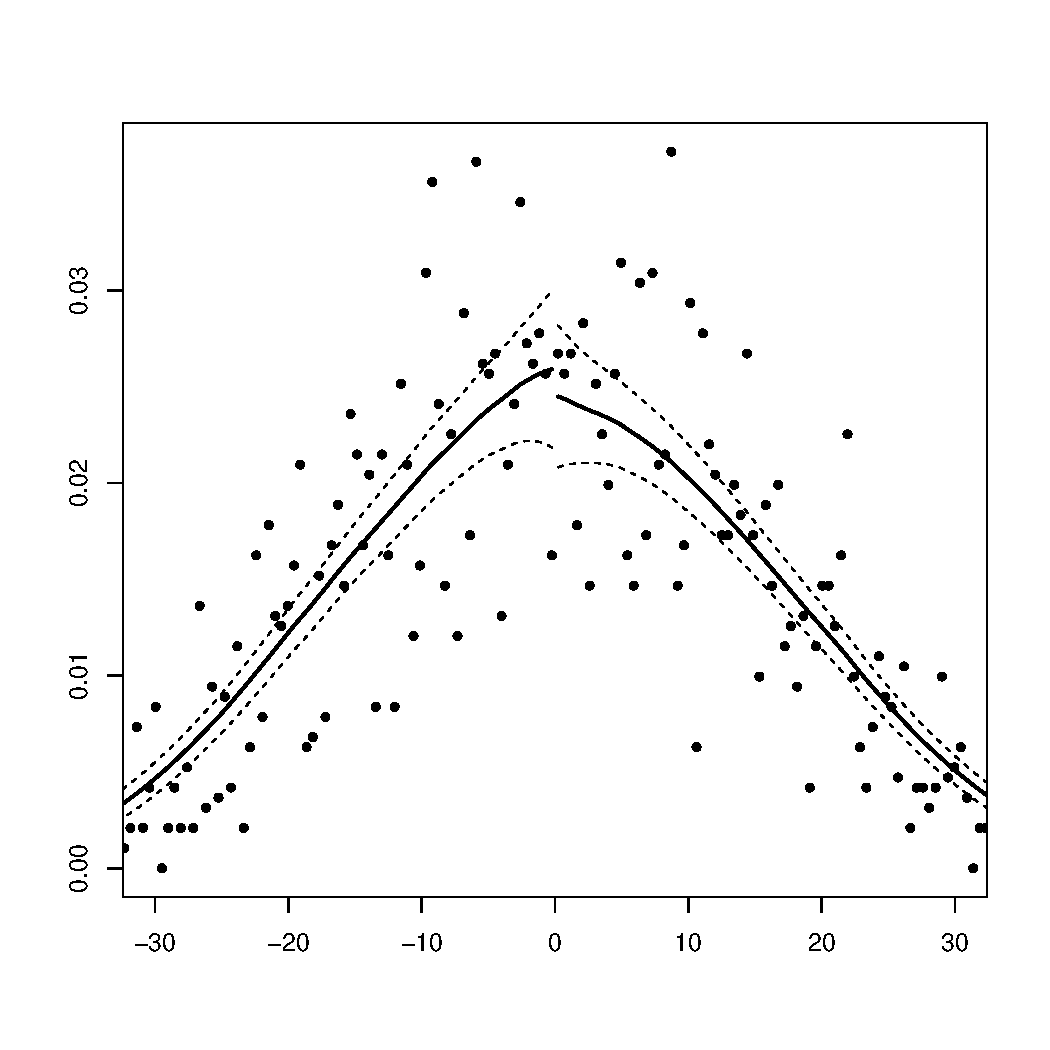
\includegraphics[width=1\linewidth]{figure/unnamed-chunk-5-1} 

\end{knitrout}
\end{centerfig}

\subsubsection{Part 5}
\label{rdd_lm}

Table \ref{q5} shows the regression estimates from the RDD performed. I use a bandwidth of 2.19, as suggested by the
\lstinline{IKbandwidth()} function.


% Table created by stargazer v.5.2.2 by Marek Hlavac, Harvard University. E-mail: hlavac at fas.harvard.edu
% Date and time: Wed, Mar 24, 2021 - 05:02:17 PM
\begin{table}[H] \centering 
  \caption{RDD Estimate for the Effect of Electing a Democratic Sheriff Calculated With lm()} 
  \label{q5} 
\begin{tabular}{@{\extracolsep{5pt}}lc} 
\\[-1.8ex]\hline 
\hline \\[-1.8ex] 
 & \multicolumn{1}{c}{\textit{Dependent variable:}} \\ 
\cline{2-2} 
\\[-1.8ex] & Share of Detainer Requests Complied With \\ 
\hline \\[-1.8ex] 
 Running Variable & 0.041 \\ 
  & (0.049) \\ 
  & \\ 
 Treatment & $-$0.103 \\ 
  & (0.080) \\ 
  & \\ 
 Running Variable : Treatment & $-$0.027 \\ 
  & (0.062) \\ 
  & \\ 
 Constant & 0.605$^{***}$ \\ 
  & (0.062) \\ 
  & \\ 
\hline \\[-1.8ex] 
Observations & 219 \\ 
R$^{2}$ & 0.009 \\ 
Adjusted R$^{2}$ & $-$0.005 \\ 
Residual Std. Error & 0.276 (df = 215) \\ 
F Statistic & 0.664 (df = 3; 215) \\ 
\hline 
\hline \\[-1.8ex] 
\textit{Note:}  & \multicolumn{1}{r}{$^{*}$p$<$0.1; $^{**}$p$<$0.05; $^{***}$p$<$0.01} \\ 
\end{tabular} 
\end{table} 


The estimate for the LATE is -.103.
This means that among barely decided elections, a democratic sheriff being elected was associated with a 10 percentage-point decrease in the proportion of detainer requests completed.

However, this is not statistically significant at any level - we do not have sufficient statistical evidence to suggest these results are not due to chance alone.
Accordingly, we cannot interpret this as indicative of a causal relationship between electing a democratic sheriff and the proportion of ICE detainer requests completed.

\subsubsection{Part 6}
I re-estimate the LATE using the \lstinline{RDestimate()} function, and obtain a LATE estimate of -.1497. This estimate is similarly insignificant at the $\alpha=.1$ level.
As the LATE is statistically insignificant across both models, the results that we have found do not hang on either model specification.

This estimate is slightly larger than the previous estimate because the \lstinline{RDestimate()} function estimates the LATE using a local linear regression as opposed to the normal linear regression method used above.
Looking at the share of the detainer requests approved around the cutoff, we can see that the trend is non-linear. This explains the discrepancies between the two results.

\begin{centerfig}
\caption{Share of Enforced Detainer Requests by Running Variable}
\begin{knitrout}
\definecolor{shadecolor}{rgb}{0.969, 0.969, 0.969}\color{fgcolor}
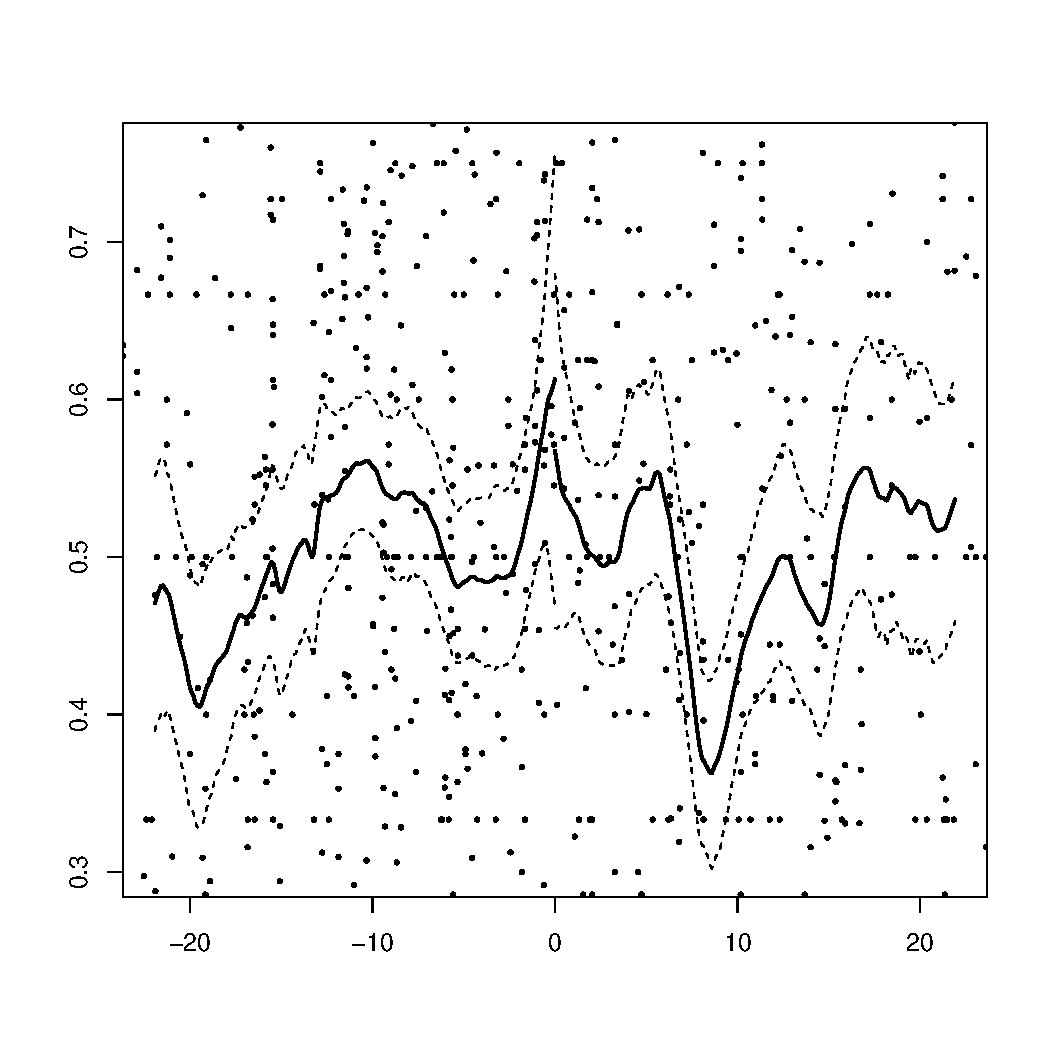
\includegraphics[width=1\linewidth]{figure/unnamed-chunk-7-1} 

\end{knitrout}
\end{centerfig}

\subsubsection{Part 7}
\begin{centerfig}
\caption{LATE Estimates Across Different Bandwidths}
\label{bandwidth}
\begin{knitrout}
\definecolor{shadecolor}{rgb}{0.969, 0.969, 0.969}\color{fgcolor}
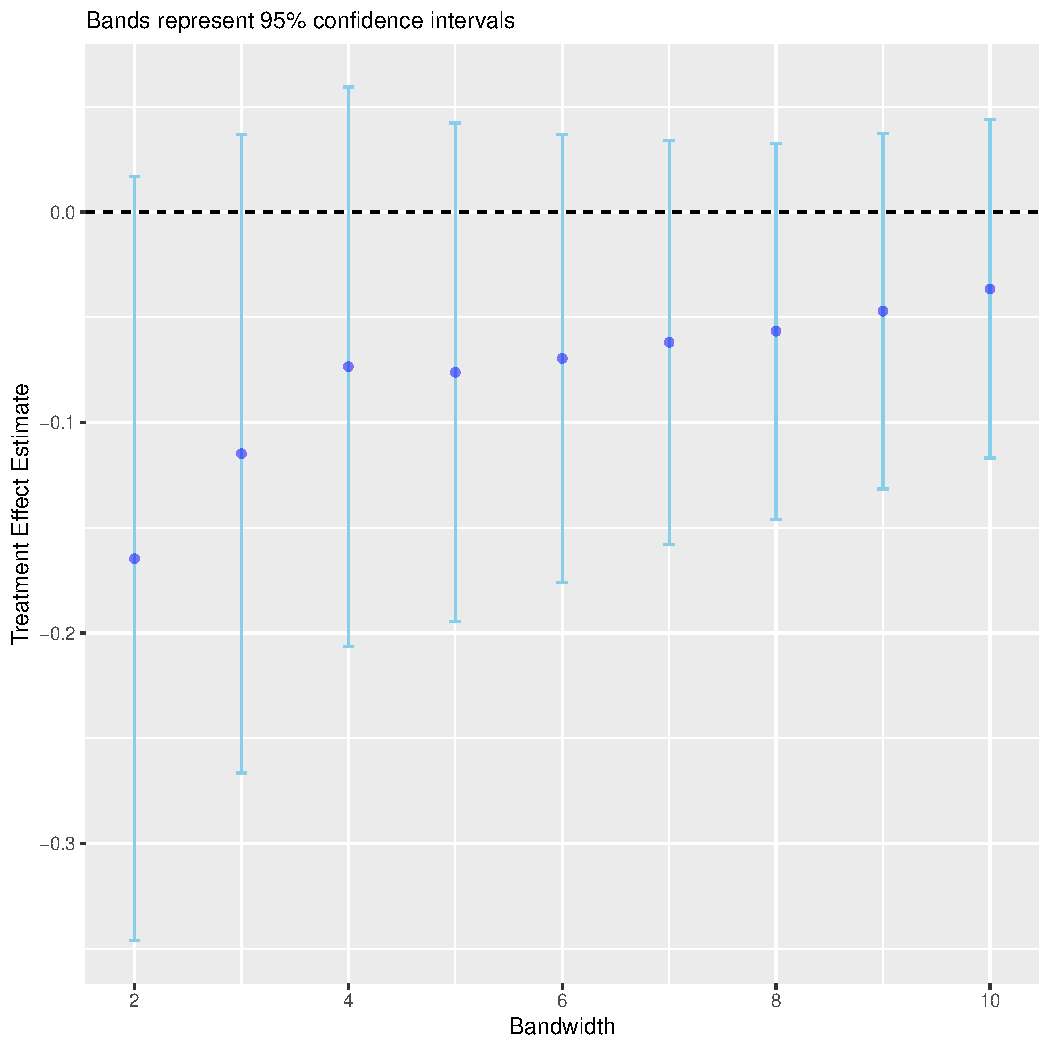
\includegraphics[width=1\linewidth]{figure/unnamed-chunk-8-1} 

\end{knitrout}
\end{centerfig}

In Figure \ref{bandwidth}, I re-estimate the LATE across bandwidths from 2 to 10.
Across all of the bandwidths, the result remains statistically insignificant.

This demonstrates that the insignificant result is robust to alternative model specifications;
the findings are not reliant on a ``knife's edge model specification" \parencite[][]{Mu_oz_2018}.
As the results from the RDD are the same over a range of plausible cutoffs, it is clear that the findings are not dependent on this specific choice of cutoff.

\subsubsection{Part 8}
Below, I report the results from a DID analysis conducted on the same dataset.

% Table created by stargazer v.5.2.2 by Marek Hlavac, Harvard University. E-mail: hlavac at fas.harvard.edu
% Date and time: Wed, Mar 24, 2021 - 05:02:18 PM
\begin{table}[H] \centering 
  \caption{} 
  \label{} 
\begin{tabular}{@{\extracolsep{5pt}}lc} 
\\[-1.8ex]\hline 
\hline \\[-1.8ex] 
 & \multicolumn{1}{c}{\textit{Dependent variable:}} \\ 
\cline{2-2} 
\\[-1.8ex] & share\_detained\_sheriff \\ 
\hline \\[-1.8ex] 
 treat & $-$0.017 \\ 
  & (0.028) \\ 
  & \\ 
 Constant & 0.398$^{***}$ \\ 
  & (0.135) \\ 
  & \\ 
\hline \\[-1.8ex] 
County Fixed Effects & Yes \\ 
Year Fixed Effects & Yes \\ 
\hline \\[-1.8ex] 
Observations & 2,056 \\ 
R$^{2}$ & 0.560 \\ 
Adjusted R$^{2}$ & 0.430 \\ 
Residual Std. Error & 0.219 (df = 1586) \\ 
F Statistic & 4.307$^{***}$ (df = 469; 1586) \\ 
\hline 
\hline \\[-1.8ex] 
\textit{Note:}  & \multicolumn{1}{r}{$^{*}$p$<$0.1; $^{**}$p$<$0.05; $^{***}$p$<$0.01} \\ 
\end{tabular} 
\end{table} 


As discussed, the RDD framework assumes that the elections near the cutoff are as good as randomly assigned.
In contrast, the DID framework relies on the parallel trends assumption that if untreated, the treated units would follow the same trends as the control units.
In this context, the parallel trends assumption would require that if left untreated, the counties which elected a democratic sheriff would follow a similar trend as those who did not.
I find this less convincing as it is less testable than the as-good-as-random assumption and because different US counties are so different that it is more difficult to imagine that they would have parallel trends in the absence of treatment.

Important to note is that the two designs return different estimands.
The DID framework estimates an ATT, while the RDD framework recovers a local average treatment effect for ``coin flip" sheriff races.

\subsubsection{Part 9}

From these analyses, we can conclude that there is no partisan difference in the enforcement of ICE detainer requests.
Multiple RDD model specifications and a DID analysis have failed to find a significant effect associated with the election of a democrat or republican on the proportion of ICE detainer requests complied with in counties with coin-toss elections.

The strength of the RDD approach is that it makes its assumptions both explicit and testable. The RDD relies on as-good-as-random assignment around the cutoff point, which can be tested using balance checks and continuity tests to test for sorting or non-random assignment around the cutoff.
As neither of these methods suggested non-random assignment, I am satisfied that the assumptions needed for the RDD to operate are met.

However, there is a clustering problem in the analysis I have conducted.
In most counties, a sheriff is elected for four years while the detainer request data is collected every year.
This creates a problem as the RDD approach treats each year of detainer data within a county as independent from the others.
However, in actual fact, if a sheriff detains a small number of people one year, it is likely that they will do so again the next year.

Failure to account for this dependency leads to artificially decreased variance in both comparison groups, resulting in artificially smaller confidence intervals and an increased chance of making a type 1 error.
As the results are not significant, this seems to have not made a difference in this case.

\subsection{Question 2}

\subsubsection{Part 1}

First, I enumerate and characterize compliers, always-takers, and never-takers:
\begin{itemize}
	\item \textbf{Compliers} are countries that would have a high level of slave exports if they were close to locations of demand for the slave trade, and a low level of slave exports if they were far away from locations of demand for the slave trade.
	\item \textbf{Always takers} are countries that would have a high level of slave exports irrespective of their distance from locations of slave-trade demand.
	\item \textbf{Never Takers:} Countries that would have a low level of slave exports irrespective of their distance from locations of slave-trade demand.
\end{itemize}

Next, I calculate the proportion of compliers
\begin{knitrout}
\definecolor{shadecolor}{rgb}{0.969, 0.969, 0.969}\color{fgcolor}\begin{kframe}
\begin{alltt}
\hlcom{#Question 2 part 1}
\hlstd{d_z_0} \hlkwb{<-} \hlkwd{mean}\hlstd{(nunn}\hlopt{$}\hlstd{high_slavery[nunn}\hlopt{$}\hlstd{low_distance}\hlopt{==}\hlnum{0}\hlstd{])}
\hlstd{d_z_1} \hlkwb{<-} \hlkwd{mean}\hlstd{(nunn}\hlopt{$}\hlstd{high_slavery[nunn}\hlopt{$}\hlstd{low_distance}\hlopt{==}\hlnum{1}\hlstd{])}
\hlstd{proportion_compliers} \hlkwb{<-} \hlstd{d_z_1} \hlopt{-} \hlstd{d_z_0}
\end{alltt}
\end{kframe}
\end{knitrout}

The proportion of compliers is equal to 11.7\%.

I now calculate the ITT effect
\begin{knitrout}
\definecolor{shadecolor}{rgb}{0.969, 0.969, 0.969}\color{fgcolor}\begin{kframe}
\begin{alltt}
\hlcom{#Question 2 part 1}
\hlcom{#Calculate ITT effect}
\hlstd{y_z_0} \hlkwb{<-} \hlkwd{mean}\hlstd{(nunn}\hlopt{$}\hlstd{ln_realgdp2000[nunn}\hlopt{$}\hlstd{low_distance}\hlopt{==}\hlnum{0}\hlstd{])}
\hlstd{y_z_1} \hlkwb{<-} \hlkwd{mean}\hlstd{(nunn}\hlopt{$}\hlstd{ln_realgdp2000[nunn}\hlopt{$}\hlstd{low_distance}\hlopt{==}\hlnum{1}\hlstd{])}
\hlstd{itt} \hlkwb{<-} \hlstd{y_z_1} \hlopt{-} \hlstd{y_z_0}
\end{alltt}
\end{kframe}
\end{knitrout}
This is is equal to -.013.

Dividing the two, I find the LATE, and calculate the p-value.
\begin{knitrout}
\definecolor{shadecolor}{rgb}{0.969, 0.969, 0.969}\color{fgcolor}\begin{kframe}
\begin{alltt}
\hlcom{#Question 2 Part 1}
\hlcom{#Calculate LATE}
\hlstd{late} \hlkwb{<-} \hlstd{itt} \hlopt{/} \hlstd{proportion_compliers}

\hlcom{# P-value}
\hlstd{p_val} \hlkwb{<-} \hlkwd{summary}\hlstd{(}\hlkwd{ivreg}\hlstd{(}\hlkwc{formula} \hlstd{= ln_realgdp2000} \hlopt{~} \hlstd{high_slavery,}
                   \hlkwc{instruments} \hlstd{=} \hlopt{~} \hlstd{low_distance,} \hlkwc{data} \hlstd{= nunn)}
                                \hlstd{)}
\end{alltt}
\end{kframe}
\end{knitrout}

The LATE is equal to the ITT divided by the proportion of compliers, or -1.13.
I calculate the p-value of this estimate as $2.45*10^{-6}$.

\subsubsection{Part 2}
Below, I use the Stargazer package \parencite[][]{Stargazer} report the results of the first stage regression.

\begin{kframe}
\begin{alltt}
\hlkwd{lm}\hlstd{(ln_export_area} \hlopt{~} \hlstd{atlantic_dist} \hlopt{+} \hlstd{indian_dist} \hlopt{+} \hlstd{saharan_dist} \hlopt{+} \hlstd{redsea_dist,} \hlkwc{data} \hlstd{= nunn)} \hlopt
        \hlkwd{stargazer}\hlstd{(}
                        \hlkwc{title} \hlstd{=} \hlstr{"First Stage Regression Results"}\hlstd{,}
                        \hlkwc{dep.var.labels} \hlstd{=} \hlkwd{c}\hlstd{(}\hlstr{"Log Slave Exports / Area"}\hlstd{),}
                        \hlkwc{covariate.labels} \hlstd{=} \hlkwd{c}\hlstd{(}\hlstr{"Atlantic Distance"}\hlstd{,}
                                                 \hlstr{"Indian Distance"}\hlstd{,}
                                                 \hlstr{"Saharan Distance"}\hlstd{,}
                                                 \hlstr{"Red Sea Distance"}\hlstd{,}
                                                 \hlstr{"Constant"}\hlstd{),}
                        \hlkwc{type}\hlstd{=}\hlstr{"latex"}\hlstd{,}
                        \hlkwc{table.placement}\hlstd{=}\hlstr{"H"}
        \hlstd{)}
\end{alltt}
\end{kframe}
% Table created by stargazer v.5.2.2 by Marek Hlavac, Harvard University. E-mail: hlavac at fas.harvard.edu
% Date and time: Wed, Mar 24, 2021 - 05:02:19 PM
\begin{table}[H] \centering 
  \caption{First Stage Regression Results} 
  \label{} 
\begin{tabular}{@{\extracolsep{5pt}}lc} 
\\[-1.8ex]\hline 
\hline \\[-1.8ex] 
 & \multicolumn{1}{c}{\textit{Dependent variable:}} \\ 
\cline{2-2} 
\\[-1.8ex] & Log Slave Exports / Area \\ 
\hline \\[-1.8ex] 
 Atlantic Distance & $-$1.314$^{***}$ \\ 
  & (0.357) \\ 
  & \\ 
 Indian Distance & $-$1.095$^{***}$ \\ 
  & (0.380) \\ 
  & \\ 
 Saharan Distance & $-$2.435$^{***}$ \\ 
  & (0.823) \\ 
  & \\ 
 Red Sea Distance & $-$0.002 \\ 
  & (0.710) \\ 
  & \\ 
 Constant & 29.110$^{***}$ \\ 
  & (6.959) \\ 
  & \\ 
\hline \\[-1.8ex] 
Observations & 52 \\ 
R$^{2}$ & 0.279 \\ 
Adjusted R$^{2}$ & 0.218 \\ 
Residual Std. Error & 3.445 (df = 47) \\ 
F Statistic & 4.545$^{***}$ (df = 4; 47) \\ 
\hline 
\hline \\[-1.8ex] 
\textit{Note:}  & \multicolumn{1}{r}{$^{*}$p$<$0.1; $^{**}$p$<$0.05; $^{***}$p$<$0.01} \\ 
\end{tabular} 
\end{table} 


\subsubsection{Part 3}


To test for weak instruments, I use the Stock and Yogo \parencite[][]{Stock_2005} test.
I test the null hypothesis that the bias resulting from weak instruments will be greater than 5\% the size of the worst-case bias from OLS against the alternative that the instruments are not weak at the  $\alpha=.05$ level.

A test statistic of 4.45 does not exceed the critical value of 16.85. Therefore, there is insignificant evidence to reject the null hypothesis that the instruments are weak.

Since the instruments are weak, the IV regression estimators will be biased towards the OLS estimators, and the standard errors we report will be too small.
Further, the estimates obtained from IV regression may be inconsistent, as the instrument induces very little variation in the treatment.

\subsubsection{Part 4}

A possible violation of the exclusion restriction is that the distance from locations of slave demand could also have an influence on the types and strength of colonial institutions built in a country.
The distance from the Saharan trade locations is heavily correlated with distance to Europe - the seat of the colonial powers.
If distance from Europe forces colonial powers to rule indirectly, a ruling system linked to stronger institutions and economic growth \parencite[][]{Iyer_2010}, then the exclusion restriction is violated.
This could plausibly be the case if the complicated logistics of direct rule from a distance encouraged colonial powers to rely on indirect rule to keep control over the colonies.

\subsubsection{Part 5}
Table \ref{secondstage} shows the second-stage regression estimates.
\begin{kframe}
\begin{alltt}
\hlstd{base_formula} \hlkwb{<-} \hlstd{ln_realgdp2000} \hlopt{~} \hlstd{ln_export_area}
\hlstd{base_instruments} \hlkwb{<-} \hlopt{~} \hlstd{redsea_dist} \hlopt{+} \hlstd{indian_dist} \hlopt{+} \hlstd{saharan_dist} \hlopt{+} \hlstd{atlantic_dist}
\hlstd{formula_colonial} \hlkwb{<-} \hlkwd{update}\hlstd{(base_formula,} \hlopt{~}\hlstd{.} \hlopt{+} \hlstd{colonial_power)}
\hlstd{instruments_colonial} \hlkwb{<-} \hlkwd{update}\hlstd{(base_instruments,} \hlopt{~}\hlstd{.} \hlopt{+} \hlstd{colonial_power)}

\hlstd{geography_controls} \hlkwb{<-} \hlopt{~} \hlstd{.} \hlopt{+} \hlstd{equator_dist} \hlopt{+} \hlstd{longitude} \hlopt{+} \hlstd{rain_min} \hlopt{+}
        \hlstd{humid_max} \hlopt{+} \hlstd{low_temp} \hlopt{+} \hlstd{ln_coastline_area}
\hlstd{formula_geo_col} \hlkwb{<-} \hlkwd{update}\hlstd{(formula_colonial, geography_controls)}
\hlstd{instruments_geo_col} \hlkwb{<-} \hlkwd{update}\hlstd{(instruments_colonial, geography_controls)}

\hlstd{excluded_countries} \hlkwb{<-} \hlkwd{c}\hlstd{(}\hlstr{"Morocco"}\hlstd{,} \hlstr{"Algeria"}\hlstd{,} \hlstr{"Tunisia"}\hlstd{,}
  \hlstr{"Libya"}\hlstd{,} \hlstr{"Egypt"}\hlstd{,}\hlstr{"Seychelles"}\hlstd{,}
  \hlstr{"Mauritius"}\hlstd{,} \hlstr{"Comoros"}\hlstd{,}
  \hlstr{"Sao Tome & Principe"}\hlstd{,} \hlstr{"Cape Verde Islands"}\hlstd{)}

\hlstd{restricted_sample} \hlkwb{<-} \hlstd{nunn} \hlopt
        \hlkwd{filter}\hlstd{(}\hlopt{!}\hlstd{country} \hlopt \hlstd{excluded_countries)}

\hlstd{model_1} \hlkwb{<-} \hlkwd{ivreg}\hlstd{(base_formula, base_instruments,} \hlkwc{data} \hlstd{= nunn)}
\hlstd{model_2} \hlkwb{<-} \hlkwd{ivreg}\hlstd{(formula_colonial, instruments_colonial,} \hlkwc{data} \hlstd{= nunn)}
\hlstd{model_3} \hlkwb{<-} \hlkwd{ivreg}\hlstd{(formula_geo_col, instruments_geo_col,} \hlkwc{data} \hlstd{= nunn)}
\hlstd{model_4} \hlkwb{<-} \hlkwd{ivreg}\hlstd{(formula_geo_col, instruments_geo_col,} \hlkwc{data} \hlstd{= restricted_sample)}

\hlkwd{stargazer}\hlstd{(model_1,model_2, model_3,model_4,}
        \hlkwc{title} \hlstd{=} \hlstr{"Second Stage Regression Results"}\hlstd{,}
        \hlkwc{covariate.labels} \hlstd{=} \hlkwd{c}\hlstd{(}\hlstr{"Log of Slave Exports / Area"}\hlstd{,} \hlstr{"Constant"}\hlstd{),}
        \hlkwc{dep.var.labels} \hlstd{=} \hlkwd{c}\hlstd{(}\hlstr{"Log Income In 2000"}\hlstd{),}
        \hlkwc{omit} \hlstd{=} \hlkwd{c}\hlstd{(}\hlstr{"colonial_power"}\hlstd{,} \hlstr{"equator_dist"}\hlstd{,} \hlstr{"longitude"}\hlstd{,}
                 \hlstr{"rain_min"}\hlstd{,} \hlstr{"humid_max"}\hlstd{,} \hlstr{"low_temp"}\hlstd{,} \hlstr{"ln_coastline_area"}\hlstd{),}
        \hlkwc{add.lines} \hlstd{=} \hlkwd{list}\hlstd{(}\hlkwd{c}\hlstd{(}\hlstr{"Colonial power fixed effects"}\hlstd{,} \hlstr{"No"}\hlstd{,} \hlstr{"Yes"}\hlstd{,} \hlstr{"Yes"}\hlstd{,} \hlstr{"Yes"}\hlstd{),}
                  \hlkwd{c}\hlstd{(}\hlstr{"Geography Controls"}\hlstd{,} \hlstr{"No"}\hlstd{,} \hlstr{"No"}\hlstd{,} \hlstr{"Yes"}\hlstd{,}\hlstr{"Yes"}\hlstd{),}
                  \hlkwd{c}\hlstd{(}\hlstr{"Restricted Sample"}\hlstd{,} \hlstr{"No"}\hlstd{,} \hlstr{"No"}\hlstd{,} \hlstr{"No"}\hlstd{,}\hlstr{"Yes"}\hlstd{)),}
        \hlkwc{label}\hlstd{=}\hlstr{"secondstage"}\hlstd{,}
        \hlkwc{table.placement}\hlstd{=}\hlstr{"H"}\hlstd{,}
        \hlkwc{type}\hlstd{=}\hlstr{"latex"}
\hlstd{)}
\end{alltt}
\end{kframe}
% Table created by stargazer v.5.2.2 by Marek Hlavac, Harvard University. E-mail: hlavac at fas.harvard.edu
% Date and time: Wed, Mar 24, 2021 - 05:02:19 PM
\begin{table}[H] \centering 
  \caption{Second Stage Regression Results} 
  \label{secondstage} 
\begin{tabular}{@{\extracolsep{5pt}}lcccc} 
\\[-1.8ex]\hline 
\hline \\[-1.8ex] 
 & \multicolumn{4}{c}{\textit{Dependent variable:}} \\ 
\cline{2-5} 
\\[-1.8ex] & \multicolumn{4}{c}{Log Income In 2000} \\ 
\\[-1.8ex] & (1) & (2) & (3) & (4)\\ 
\hline \\[-1.8ex] 
 Log of Slave Exports / Area & $-$0.208$^{***}$ & $-$0.201$^{***}$ & $-$0.286$^{*}$ & $-$0.221$^{***}$ \\ 
  & (0.053) & (0.047) & (0.153) & (0.076) \\ 
  & & & & \\ 
 Constant & 7.811$^{***}$ & 7.716$^{***}$ & 8.602$^{***}$ & 7.948$^{***}$ \\ 
  & (0.204) & (0.579) & (2.525) & (1.513) \\ 
  & & & & \\ 
\hline \\[-1.8ex] 
Colonial power fixed effects & No & Yes & Yes & Yes \\ 
Geography Controls & No & No & Yes & Yes \\ 
Restricted Sample & No & No & No & Yes \\ 
Observations & 52 & 52 & 52 & 42 \\ 
R$^{2}$ & 0.127 & 0.342 & 0.041 & 0.511 \\ 
Adjusted R$^{2}$ & 0.110 & 0.220 & $-$0.322 & 0.284 \\ 
Residual Std. Error & 0.779 (df = 50) & 0.729 (df = 43) & 0.949 (df = 37) & 0.612 (df = 28) \\ 
\hline 
\hline \\[-1.8ex] 
\textit{Note:}  & \multicolumn{4}{r}{$^{*}$p$<$0.1; $^{**}$p$<$0.05; $^{***}$p$<$0.01} \\ 
\end{tabular} 
\end{table} 


The regression estimate of -.208 in the first model is the estimated LATE. Important to note is that this LATE is the average of the causal effects across the entire treatment range, weighted by the proportion of compliers at each level of treatment.
This effect is significant and indicates a negative causal relationship between slave exports and economic development.

\subsubsection{Part 6}
Nunn likely included the models in columns 2 and 3 as the assumptions for instrumental variables require all instruments to be as good as randomly assigned, conditional on covariates.

Conditioning on covariates makes this assumption more plausible, especially as it seems that the assignment of the instruments would not be as good as random without conditioning for some of these factors.
As an example, the colonial power that controlled the country could affect the number of slaves exported per area if one colonial power extracted more slaves than others.
If the colonial power controlling a colony is also correlated with the distances from locations of demand, then the independence assumption is not met and a selection bias is still present.

\subsubsection{Part 7}
Taken together, these results suggest that being selected into the slave trade significantly decreases the income of a country in the year 2000.
Multiple presented models show that the significance of the findings is not dependent on a single model.
Although I have highlighted a potential worries about weak instruments, I take the evidence as a whole to be convincing.

\newpage
\section{Part B: Research Proposal}
\subsection{Introduction}

Human-made schedule changes such as time zones or daylight savings time disrupt our circadian rhythms and change the hours we spend outside of our houses.
Public health research has investigated the effects of moving to daylight savings time on motor and industrial accidents \parencites{Holland_2000}{Smith_2016}{Varughese_2001}.
Other research has stressed the effects of living on the eastern versus western side of a timezone border on voter turnout, sleep, and self-reported wellbeing \parencites[][]{Holbein_2019}{Giuntella_2019}.

For my research proposal, I choose to investigate the effect of switching from the western to the eastern side of a timezone on school performance.
The underlying causal theory is that being on the western side of a timezone means students must wake up earlier relative to the solar time where they live.
This contributes to both a lack of sleep and means that students take classes in what are effectively earlier hours of the morning than they otherwise would, decreasing engagement.
To estimate the effect of switching time zones, on academic performance, I suggest using a difference-in-differences approach to estimate the effect on standardized test scores switching time zones had for a group of Indiana counties that switched time zones in 2007.

\subsection{Context and Data}

In 2006, eight counties on the western side of Indiana switched from eastern time to central time \parencite{tzchanges}.
Six of these counties switched back to eastern time in 2007, while two still use central time today.
These variations in time zones provide the basis for a difference in difference study on the effects of time zones on academic performance.

To measure academic performance, I propose using scores on the ISTEP, a standardized test Indiana students must take each year. School-level ISTEP score data is publicly available from the Indiana Department of Education website.

\subsection{Methods}
To test for a causal effect, I suggest a difference in differences model. This approach will allow us to recover the average treatment effect of switching time zones on school performance among the counties that switched time zones.

A DID model is appropriate as it is impossible to randomize the assignment of time zones. Thus, the only way forwards is to attempt to construct counterfactuals for the treatment units by propagating the trends of the control units forwards.
The DID model cancels out the effects of time-invariant omitted variables, escaping the problem of selection bias, provided that the comparison groups follow parallel trends.
This means that even though the groups that selected into central time in 2007 differ from the rest of the state in that they are on the eastern border and often more rural than other counties, as long as they follow the same trends as other counties in the state, we can still estimate the causal effect of their decision to switch time zones.

As the data is observational, and the treated units represent a somewhat typical set of US counties, I expect the causal estimates recovered from this model to be relatively externally valid, provided that the assumptions of the model are met.

\section{Model Specification}

As all of the counties made the initial switch into the central time zone at the same time, I would instrument the DID approach using the following regression equation:

$$Y_i=\alpha + \beta_1D_i + \beta_2T_i + \beta_3(T_i * D_i)$$
Where $Y_i$ represents the average ISTEP scores at each school, $D_i$ represents whether each school was treated, and $T_i$ represents the time period at which the measurement was taken.
$\beta_3$ represents the ATT, or the treatment effect amongst those schools that switched time zones.

The treatment assignment occurs at the county-level, while test scores are typically measured at the school level. This could cause a problem if errors within counties are correlated, i.e., strong performance of a school in one part of a county predicts strong performance of a school in a different part of that county.
As such, I would make sure to estimate cluster-robust standard errors to ensure that the standard errors are not artificially reduced.

\section{Assumptions and checks}
The main assumption of the difference-in-differences approach is that of parallel trends. This assumption stipulates that if the treatment group (the group of counties that switched time zones) were to have received the control assignment (not switching), they would have followed the same trend as the control group (the other Indiana counties).
As this is an assumption about the behavior of counterfactuals, it can be justified but not verified.

I will support the parallel trends assumption with a visual inspection of the trends for the two counties over time. Testing data for the ISTEP is available from before 1999, so there are many time periods over which to check the parallel trends assumption.

\subsection{Two Potential Pitfalls}
The main worry of this approach is that it could potentially not have the statistical power / sample size needed to detect a true effect. To my knowledge, there have been no previous studies on time-zone selection and academic performance, making it difficult to justify a plausible effect size to use for power analysis.
Plausibly, a 20 minute reduction in sleep could result in a .75\% worse test performance.
Power analysis using the variance in the actual data is needed to see whether such an effect could be detected.

If statistical power is an issue, then an RDD design could be used to estimate the effect of switching time zones on SAT / ACT test scores across the entire nation, taking whether a county is on the bare right-side or bare left-side of a time zone border as randomly assigned.
This approach has been previously used to estimate the effects of living on one side of a time zone border or another on voter turnout, sleep, and various other health outcomes \parencites{Giuntella_2019}{Holbein_2019}.

Another worry is that some students may attend school districts outside of their timezones by traveling across county lines for school.
This treatment spillover would likely bias estimates of the causal effect towards zero, as it undermines the distinctions between treatment and control groups.
The degree to which spillover is a problem can be tested when analyzing the data - if many students do transfer into schools in the eastern timezone, then this spells a problem for the experiment. If the number of transfers are minimal, then the estimates of the causal effects might be slightly biased towards zero but the results of the study itself will not necessarily be undermined.

\newpage
\printbibliography
\section{Appendix: R code}

\lstinputlisting[language=R]{final.R}
\end{document}


